\documentclass[12pt, a4paper]{article}

% ========================
% PACOTES
% ========================
\usepackage[utf8]{inputenc}
\usepackage[T1]{fontenc}
\usepackage[brazilian]{babel}
\usepackage{geometry}
\usepackage{graphicx}
\usepackage{hyperref}
\usepackage{tabularx}
\usepackage{booktabs}
\usepackage{enumitem}
\usepackage{indentfirst}
\usepackage{titlesec}
\usepackage{fancyhdr}
\usepackage{longtable}
\usepackage{array}
\usepackage{float}
\usepackage{adjustbox}  % Permite expandir as imagens simetricamente para fora da margem de escrita

\geometry{left=3cm, right=2cm, top=3cm, bottom=2cm}

\hypersetup{
    colorlinks=true,
    linkcolor=black,
    urlcolor=blue,
    citecolor=black
}

% ========================
% INÍCIO DO DOCUMENTO
% ========================
\begin{document}

% ========================
% CAPA
% ========================
\begin{titlepage}
\centering

\textbf{UNIVERSIDADE FEDERAL DE SERGIPE (UFS)}\\
\textbf{CENTRO DE CIÊNCIAS EXATAS E TECNOLOGIA (CCET)}\\
\textbf{DEPARTAMENTO DE COMPUTAÇÃO (DCOMP)}\\
\textbf{ENGENHARIA DE SOFTWARE -- COMP0503}\\

\vspace{3cm}

{\LARGE \textbf{Descrição Arquitetural do\\Sistema de Intermediação de Brechós}}\\

\vspace{1cm}

{\large Conforme ISO/IEC/IEEE 42010:2022}\\

\vspace{3cm}

Caroline Santos, Beatriz Eduão, Ian Daniel\\
João Pedro M., Arthur Soares, Luiz Manoel\\

\vspace{2cm}

Prof. Dr. Michel Soares\\

\vfill

Aracaju -- SE\\
23 de junho de 2026

\end{titlepage}

\newpage

% ========================
% SUMÁRIO
% ========================
\tableofcontents
\newpage

% ================================================================
% SEÇÃO 1 — IDENTIFICAÇÃO DA ARCHITECTURE DESCRIPTION
% ================================================================
\section{Identificação da Architecture Description}

Este documento constitui a \textit{Architecture Description} (AD) do Sistema de Intermediação de Brechós, elaborada em conformidade com a norma ISO/IEC/IEEE 42010:2022.

% ----------------------------------------
\subsection{Entity of Interest}

A entidade de interesse (\textit{Entity of Interest}) desta AD é o \textbf{Sistema de Intermediação de Brechós} --- uma plataforma web no modelo C2C (\textit{Consumer-to-Consumer}) destinada à compra e venda de peças de vestuário usadas. O sistema permite que usuários atuem simultaneamente como compradores e vendedores, intermediando o processo de anúncio, busca, comunicação, pagamento e acompanhamento de pedidos.

O sistema é classificado como uma aplicação web de domínio comercial, independente e totalmente contida.

% ----------------------------------------
\subsection{Escopo da Architecture Description}

Esta AD cobre a arquitetura de software do sistema em sua totalidade, abrangendo:

\begin{itemize}[noitemsep]
    \item a organização dos componentes de software e suas interfaces;
    \item as decisões arquiteturais significativas e suas justificativas;
    \item o mapeamento dos componentes nos ambientes de execução;
    \item as táticas arquiteturais adotadas para atender aos atributos de qualidade.
\end{itemize}

Esta AD \textbf{não} cobre: o design detalhado de interfaces gráficas (UI/UX) nem a implementação interna dos serviços externos integrados (código-fonte do Mercado Pago, Vercel Blob, Melhor Envio ou ViaCEP). A forma de integração com esses serviços (protocolos, padrões de comunicação e contratos de API), bem como a infraestrutura utilizada para hospedagem e execução do sistema, fazem parte do escopo desta AD.

% ----------------------------------------
\subsection{Ambiente (\textit{Environment})}

Conforme a ISO/IEC/IEEE 42010:2022, o ambiente compreende todas as influências sobre a entidade de interesse. O Sistema de Intermediação de Brechós opera sob as seguintes influências:

\subsubsection{Influências Técnicas}
\begin{itemize}[noitemsep]
    \item Plataforma web acessível via navegadores modernos, com HTML renderizado no servidor e melhoria progressiva via HTMX.
    \item Dependência de conectividade à internet para todas as operações.
    \item Execução da aplicação Go em um processo HTTP único, com páginas SSR, API JSON e arquivos estáticos servidos pelo próprio backend. Em ambiente local, o PostgreSQL e as migrações são orquestrados por Docker Compose.
    \item Integração com serviços externos: gateway de pagamentos Mercado Pago (REST/HTTPS), armazenamento de mídia Vercel Blob, cotação de frete Melhor Envio, consulta de CEP ViaCEP e banco de dados relacional PostgreSQL.
    \item Comunicação cliente-servidor via HTTPS. Conversas e notificações são persistidas no PostgreSQL e acessadas por requisições HTTP/HTMX; não há servidor WebSocket dedicado nem envio SMTP implementado nesta versão.
    \item Stack tecnológica de implementação definida para o ciclo atual: Go (Golang) no backend, templates HTML renderizados no servidor, HTMX versionado localmente, JavaScript pontual para interações de interface e PostgreSQL para persistência.
\end{itemize}

\subsubsection{Influências Operacionais}
\begin{itemize}[noitemsep]
    \item O sistema deve suportar acesso contínuo de múltiplos usuários simultâneos, com exceção de períodos de manutenção programada.
    \item Adaptação exclusiva ao idioma português brasileiro (PT-BR), moeda Real (R\$) e formatos locais de data e endereço.
    \item Upload de imagens limitado a 5MB por arquivo e 2 a 5 imagens por anúncio; o catálogo público utiliza carregamento paginado/progressivo.
\end{itemize}

\subsubsection{Influências Regulatórias e Legais}
\begin{itemize}[noitemsep]
    \item Lei Geral de Proteção de Dados --- LGPD (Lei n\textsuperscript{o} 13.709/2018): armazenamento e tratamento de dados pessoais e sensíveis.
    \item Código de Defesa do Consumidor --- CDC (Lei n\textsuperscript{o} 8.078/1990): transparência e responsabilidade nas relações de consumo.
    \item Marco Civil da Internet (Lei n\textsuperscript{o} 12.965/2014): proteção dos direitos dos usuários no ambiente digital.
    \item Presença obrigatória de Termos de Uso e Políticas de Privacidade na plataforma.
\end{itemize}

\subsubsection{Influências Organizacionais}
\begin{itemize}[noitemsep]
    \item Projeto desenvolvido no âmbito da disciplina COMP0503 --- Engenharia de Software, Universidade Federal de Sergipe, sob orientação do Prof. Dr. Michel Soares.
    \item Equipe composta por 6 desenvolvedores com restrições de cronograma acadêmico.
    \item Padronização de código-fonte e documentação atualizada como requisitos organizacionais.
\end{itemize}

% ----------------------------------------
\subsection{Referências Normativas}

\begin{itemize}[noitemsep]
    \item ISO/IEC/IEEE 42010:2022 --- \textit{Software, systems and enterprise --- Architecture description.}
    \item IEEE Std 830-1998 --- \textit{IEEE Recommended Practice for Software Requirements Specifications.}
    \item Bass, L.; Clements, P.; Kazman, R. \textit{Software Architecture in Practice.} 3rd ed. Addison-Wesley, 2012.
    \item Kruchten, P. The 4+1 View Model of Architecture. \textit{IEEE Software}, v.~12, n.~6, p.~42--50, 1995.
    \item Clements, P. et al. \textit{Documenting Software Architectures: Views and Beyond.} 2nd ed. Addison-Wesley, 2010.
\end{itemize}

% ----------------------------------------
\subsection{Glossário}

\begin{longtable}{|p{4.5cm}|p{10cm}|}
\hline
\textbf{Termo} & \textbf{Definição} \\
\hline
\endfirsthead
\hline
\textbf{Termo} & \textbf{Definição} \\
\hline
\endhead
Architecture Description (AD) & Artefato utilizado para expressar a arquitetura de uma entidade de interesse, conforme ISO/IEC/IEEE 42010:2022. \\
\hline
Entity of Interest & Entidade cuja arquitetura está sendo descrita --- neste caso, o Sistema de Intermediação de Brechós. \\
\hline
Stakeholder & Indivíduo, equipe ou organização com interesses no sistema. \\
\hline
Concern & Qualquer interesse no sistema: expectativa, necessidade, objetivo, restrição, atributo de qualidade, risco. \\
\hline
Architecture Viewpoint & Conjunto de convenções para construir, interpretar e analisar um tipo de Architecture View. \\
\hline
Architecture View & Representação da arquitetura sob a perspectiva de um conjunto de concerns, governada por viewpoint. \\
\hline
Model Kind & Convenções para um tipo de modelo arquitetural (linguagem, notação, técnicas analíticas). \\
\hline
Architecture Decision & Decisão de design significativa que afeta \textit{elements} da AD e pertence a um ou mais concerns. \\
\hline
Architecture Rationale & Justificativa, explicação ou raciocínio sobre decisões arquiteturais tomadas e alternativas descartadas. \\
\hline
Correspondence & Relação entre elementos da AD (rastreabilidade, consistência, refinamento). \\
\hline
Correspondence Rule & Regra que governa e verifica correspondências dentro ou entre ADs. \\
\hline
C2C & \textit{Consumer-to-Consumer} --- modelo de comércio eletrônico entre consumidores. \\
\hline
SRS & \textit{Software Requirements Specification} --- Especificação de Requisitos de Software. \\
\hline
\end{longtable}

% ================================================================
% SEÇÃO 2 — STAKEHOLDERS E CONCERNS
% ================================================================
\section{Stakeholders e Concerns}

Conforme a ISO/IEC/IEEE 42010:2022, uma Architecture Description deve identificar os stakeholders cujas preocupações são consideradas fundamentais para a arquitetura, bem como os concerns associados a cada um deles. Esta seção apresenta os stakeholders do Sistema de Intermediação de Brechós e os concerns arquiteturalmente significativos, com ênfase nos atributos de qualidade de desempenho, escalabilidade, segurança e disponibilidade.

% ----------------------------------------
\subsection{Identificação dos Stakeholders}

\begin{longtable}{|p{3.5cm}|p{3cm}|p{7.5cm}|}
\hline
\textbf{Stakeholder} & \textbf{Papel (42010)} & \textbf{Descrição} \\
\hline
\endfirsthead
\hline
\textbf{Stakeholder} & \textbf{Papel (42010)} & \textbf{Descrição} \\
\hline
\endhead
Comprador & \textit{User} & Usuário que pesquisa, filtra e adquire peças de vestuário na plataforma. Interage com o sistema por meio do feed de anúncios, carrinho de compras, chat e acompanhamento de pedidos. \\
\hline
Vendedor & \textit{User} & Usuário que publica anúncios, gerencia itens e realiza envios. Recebe repasses financeiros após a confirmação de entrega. Um usuário pode exercer ambos os papéis (comprador e vendedor) simultaneamente. \\
\hline
Equipe de Desenvolvimento & \textit{Developer, Builder, Maintainer} & Responsável pela implementação, testes e manutenção do código-fonte do sistema. \\
\hline
Equipe de Infraestrutura & \textit{Operator} & Responsável pela implantação, operação e monitoramento do sistema em ambiente de produção, incluindo a infraestrutura em nuvem. \\
\hline
Product Owner & \textit{Acquirer, Owner} & Responsável por avaliar os resultados. No contexto deste projeto, esse papel é exercido pelo Prof. Dr. Michel Soares. \\
\hline
\end{longtable}

% ----------------------------------------
\subsection{Identificação dos Concerns}

A ISO/IEC/IEEE 42010:2022 define \textit{concern} como qualquer interesse no sistema --- expectativas, necessidades, objetivos, restrições, atributos de qualidade ou riscos.

Os concerns identificados para esta AD estão organizados em duas categorias: concerns de qualidade priorizados e concerns contextuais.

\subsubsection{Concerns de Qualidade (Atributos de Qualidade)}

Estes são os concerns prioritários desta Architecture Description.

\vspace{0.5cm}

\noindent\textbf{CQ01 --- Desempenho}

O desempenho diz respeito ao volume de trabalho que o sistema deve executar em um período de tempo e aos limites de tempo de resposta que devem ser respeitados. No Sistema de Intermediação de Brechós, o desempenho é crítico em três pontos: a renderização do catálogo, o processamento transacional do checkout e a atualização das conversas/notificações via requisições HTTP.

\begin{longtable}{|p{4.5cm}|p{10cm}|}
\hline
\textbf{Métrica} & \textbf{Especificação} \\
\hline
Tempo de resposta (Response Time) & 95\% das requisições HTTP devem ser respondidas pelo servidor em até 500ms. Nenhuma requisição deve exceder 3 segundos. \\
\hline
Throughput & O sistema deve processar no mínimo 100 requisições por segundo no pico de utilização, considerando operações de leitura (feed, busca) e escrita (criação de anúncios, compras). \\
\hline
Atualização de conversas & Mensagens enviadas no pedido devem ser persistidas no PostgreSQL e disponibilizadas ao destinatário por requisições HTTP/HTMX, sem infraestrutura WebSocket dedicada. \\
\hline
Renderização inicial & O feed de anúncios deve ser renderizado no navegador do usuário em até 3 segundos na primeira carga. \\
\hline
\end{longtable}

\noindent As táticas arquiteturais adotadas para atender a este concern são detalhadas na Seção 5 (Architecture Decisions e Rationale).

\vspace{0.5cm}

\noindent\textbf{CQ02 --- Escalabilidade}

A escalabilidade refere-se à capacidade do sistema de manter seu desempenho quando a demanda aumenta, seja em volume de requisições, sessões simultâneas ou tamanho dos dados armazenados. A implementação atual prioriza simplicidade operacional acadêmica: um backend Go stateless em relação ao processo, persistência centralizada no PostgreSQL, arquivos públicos no Vercel Blob e paginação das listagens. O crescimento horizontal depende de múltiplas instâncias compartilhando o mesmo banco e os mesmos serviços externos.

\begin{longtable}{|p{4.5cm}|p{10cm}|}
\hline
\textbf{Dimensão} & \textbf{Decisão Arquitetural} \\
\hline
Servidor sem estado de sessão em memória & A aplicação não mantém sessão em memória local. A sessão do navegador é transportada por cookie \textit{HttpOnly}, \textit{SameSite=Lax} e \textit{Secure} em HTTPS, enquanto os dados persistentes ficam no PostgreSQL. Clientes de API podem solicitar transporte Bearer explicitamente. \\
\hline
Carga de requisições & Operações de leitura intensiva (feed de anúncios, busca e filtragem) devem utilizar caching para reduzir a carga sobre o banco de dados. A paginação de resultados (20 a 30 registros por requisição) limita o volume de dados trafegados por chamada. \\
\hline
Volume de dados & As consultas ao banco de dados utilizam filtros de categoria, tamanho, faixa de preço, status e paginação. Arquivos de mídia são armazenados no Vercel Blob, evitando crescimento do banco de dados relacional com binários. \\
\hline
\end{longtable}

\noindent As táticas arquiteturais adotadas para viabilizar a escalabilidade são detalhadas na Seção 5 (Architecture Decisions e Rationale).

\vspace{0.5cm}

\noindent\textbf{CQ03 --- Segurança}

A segurança abrange a capacidade do sistema de proteger dados e recursos contra acessos não autorizados, garantindo autenticação, autorização e criptografia.

\begin{longtable}{|p{4.5cm}|p{10cm}|}
\hline
\textbf{Métrica} & \textbf{Especificação} \\
\hline
Autenticação & O sistema deve verificar a identidade dos usuários por meio de credenciais (e-mail/CPF e senha). Senhas devem ser armazenadas com hash bcrypt (custo mínimo 10). \\
\hline
Autorização & Usuários autenticados devem ter acesso restrito às operações permitidas ao seu papel. Um vendedor só pode editar ou excluir anúncios próprios. Um comprador só pode acessar pedidos próprios. \\
\hline
Criptografia & Todas as comunicações cliente-servidor devem utilizar TLS 1.2 ou superior. Dados completos de cartão não são armazenados no sistema; quando o pagamento real está habilitado, a tokenização ocorre pelo SDK do Mercado Pago e a cobrança é confirmada por \textit{webhook}. \\
\hline
Conformidade LGPD & O sistema deve permitir que o usuário solicite a exclusão de seus dados pessoais. Dados sensíveis (CPF, endereço, dados bancários) devem ser armazenados com criptografia em repouso. \\
\hline
Sessão do navegador & A sessão web é mantida em cookie \textit{HttpOnly}, \textit{SameSite=Lax} e \textit{Secure} em HTTPS. Requisições mutáveis autenticadas por cookie passam por verificação de origem para reduzir risco de CSRF. \\
\hline
\end{longtable}

\noindent As táticas arquiteturais adotadas para atender a este concern são detalhadas na Seção 5 (Architecture Decisions e Rationale).

\vspace{0.5cm}

\noindent\textbf{CQ04 --- Disponibilidade}

A disponibilidade refere-se à probabilidade de que o sistema esteja pronto para executar suas tarefas quando o usuário necessitar. Devido à escolha de infraestrutura gratuita (CC02), a arquitetura não pode garantir SLAs de \textit{uptime} de 99,99\% (como em provedores AWS \textit{Enterprise}). Portanto, a abordagem arquitetural foca em minimizar o MTTR (\textit{Mean Time to Repair}) e em aplicar táticas de tolerância a falhas.

\begin{longtable}{|p{4.5cm}|p{10cm}|}
\hline
\textbf{Métrica / Tática} & \textbf{Especificação Aplicada} \\
\hline
Recuperação de Falhas (Processo Go) & A aplicação centraliza API, SSR e arquivos estáticos em um processo Go simples de reiniciar e com endpoints de liveness/readiness (\texttt{/saude} e \texttt{/saude/prontidao}) para monitoramento operacional. \\
\hline
Recuperação de Falhas (Degradação Graciosa) & Tática aplicada às integrações externas. Na ausência de credenciais do Melhor Envio, o checkout usa frete fixo; na ausência de credenciais do Mercado Pago, o sistema usa provedor de pagamento simulado para manter o fluxo acadêmico executável. \\
\hline
Recuperação de Falhas (\textit{Rollback} e Transações) & Tática aplicada ao checkout. A reserva de anúncios, criação da compra, pedidos, pagamento e liberação de itens em caso de recusa/expiração são controladas por transações no PostgreSQL, reduzindo inconsistências entre carrinho, estoque e pagamento. \\
\hline
\end{longtable}

\noindent As táticas arquiteturais adotadas para atender a este concern são detalhadas na Seção 5 (Architecture Decisions e Rationale).

% ----------------------------------------
\subsubsection{Concerns Contextuais}

\begin{longtable}{|p{1.2cm}|p{4.5cm}|p{8.8cm}|}
\hline
\textbf{ID} & \textbf{Concern} & \textbf{Descrição} \\
\hline
\endfirsthead
\hline
\textbf{ID} & \textbf{Concern} & \textbf{Descrição} \\
\hline
\endhead
CC01 & Propósito do sistema & Intermediar de forma organizada e segura o processo de compra e venda de peças de vestuário usadas entre consumidores, promovendo os brechós como experiência digital intuitiva. \\
\hline
CC02 & Viabilidade de construção e implantação & O sistema é desenvolvido por uma equipe de 6 integrantes em contexto acadêmico, com restrições de cronograma. Essas restrições influenciaram a escolha por backend Go único, SSR/HTMX, Docker Compose para PostgreSQL local, integrações com fallback e ausência de etapa de build frontend. \\
\hline
CC03 & Manutenibilidade e evolvabilidade & O sistema deve ser estruturado de forma que permita a adição de novas funcionalidades e a correção de defeitos com impacto controlado sobre os demais componentes. Embora não seja um atributo de qualidade priorizado nesta AD, a organização em camadas e o baixo acoplamento entre componentes favorecem a manutenibilidade. \\
\hline
CC04 & Riscos e impactos ao longo do ciclo de vida & Os principais riscos identificados incluem: indisponibilidade de serviços externos (Mercado Pago, Melhor Envio, ViaCEP e Vercel Blob), imagens órfãs após upload abandonado, necessidade futura de reconciliação de pagamentos pendentes e exposição de dados pessoais em desconformidade com a LGPD. \\
\hline
\end{longtable}

% ----------------------------------------
\subsection{Matriz Concern $\times$ Stakeholder}

\begin{longtable}{|p{3.5cm}|c|c|c|c|c|}
\hline
\textbf{Concern} & \rotatebox{70}{\textbf{Comprador}} & \rotatebox{70}{\textbf{Vendedor}} & \rotatebox{70}{\textbf{Eq. Desenvolvimento}} & \rotatebox{70}{\textbf{Eq. Infraestrutura}} & \rotatebox{70}{\textbf{Product Owner}} \\
\hline
\endfirsthead
\hline
\textbf{Concern} & \rotatebox{70}{\textbf{Comprador}} & \rotatebox{70}{\textbf{Vendedor}} & \rotatebox{70}{\textbf{Eq. Desenvolvimento}} & \rotatebox{70}{\textbf{Eq. Infraestrutura}} & \rotatebox{70}{\textbf{Product Owner}} \\
\hline
\endhead
\textbf{CQ01 -- Desempenho} & $\bullet$ & $\bullet$ & $\bullet$ & $\bullet$ & $\bullet$ \\
\hline
\textbf{CQ02 -- Escalabilidade} & & & & $\bullet$ & $\bullet$ \\
\hline
\textbf{CQ03 -- Segurança} & $\bullet$ & $\bullet$ & $\bullet$ & $\bullet$ & $\bullet$ \\
\hline
\textbf{CQ04 -- Disponibilidade} & $\bullet$ & $\bullet$ & & $\bullet$ & $\bullet$ \\
\hline
CC01 -- Propósito & $\bullet$ & $\bullet$ & & & $\bullet$ \\
\hline
CC02 -- Viabilidade & & & $\bullet$ & $\bullet$ & $\bullet$ \\
\hline
CC03 -- Manutenibilidade & & & $\bullet$ & & $\bullet$ \\
\hline
CC04 -- Riscos & $\bullet$ & $\bullet$ & $\bullet$ & $\bullet$ & $\bullet$ \\
\hline
\end{longtable}

% ================================================================
% SEÇÃO 3 — ARCHITECTURE VIEWPOINTS
% ================================================================
\section{Architecture Viewpoints}

Conforme a ISO/IEC/IEEE 42010:2022, um \textit{Architecture Viewpoint} é um conjunto de convenções para construir, interpretar, utilizar e analisar um tipo de \textit{Architecture View}. Cada viewpoint enquadra (\textit{frames}) um conjunto específico de concerns. Esta AD adota quatro viewpoints fundamentais e um integrado (+1), mantendo o escopo estritamente focado em elements exclusivos da arquitetura global.

% ----------------------------------------
\subsection{VP1 --- Viewpoint Lógico}

\begin{longtable}{|p{4.5cm}|p{10cm}|}
\hline
\textbf{Nome} & Viewpoint Lógico \\
\hline
\textbf{Concerns enquadrados} & CC01 (Propósito do sistema), CQ03 (Segurança --- regras de autorização) \\
\hline
\textbf{Stakeholders interessados} & Comprador, Vendedor, Equipe de Desenvolvimento, Product Owner \\
\hline
\textbf{Model Kinds próprios} & MK1 --- Modelo Conceitual de Domínio \\
\hline
\textbf{Referências} & Kruchten (1995), Bass et al. (2012), UML 2.5 Specification \\
\hline
\end{longtable}

\noindent\textbf{MK1 --- Modelo Conceitual de Domínio}
\begin{longtable}{|p{4.5cm}|p{10cm}|}
\hline
\textbf{Linguagem/Notação} & UML 2.5 --- Diagrama de Classes (Alto Nível) \\
\hline
\textbf{Elementos utilizados} & Entidades conceituais (\texttt{<<class>>}), associações, composições e multiplicidades. (Ocultam-se atributos, enumerações e métodos para preservar a abstração arquitetural). \\
\hline
\textbf{Ferramenta} & Draw.io ou Astah \\
\hline
\textbf{Propósito} & Representar a estrutura conceitual do domínio do sistema, identificando as entidades e os relacionamentos semânticos que sustentam as regras de negócio da intermediação C2C, sem viés de implementação. \\
\hline
\end{longtable}

\paragraph{Referências Externas Complementares:} O projeto não utiliza a modelagem Entidade-Relacionamento (ER) clássica como visão arquitetural principal. A definição do esquema físico de banco de dados e as amarrações de chaves no PostgreSQL são tratadas como artefatos de \textit{Design de Software} e implementadas por migrações SQL e adaptadores Data Mapper com pgx, sem ORM. Portanto, esses detalhes técnicos foram intencionalmente abstraídos desta Descrição Arquitetural para focar puramente na estrutura conceitual de alto nível.

% ----------------------------------------
\subsection{VP2 --- Viewpoint de Desenvolvimento}

\begin{longtable}{|p{4.5cm}|p{10cm}|}
\hline
\textbf{Nome} & Viewpoint de Desenvolvimento \\
\hline
\textbf{Concerns enquadrados} & CC03 (Manutenibilidade e evolvabilidade), CC02 (Viabilidade de construção) \\
\hline
\textbf{Stakeholders interessados} & Equipe de Desenvolvimento \\
\hline
\textbf{Model Kinds próprios} & MK2 --- Diagrama de Camadas \\
\hline
\textbf{Referências} & Parnas (1972), Dijkstra (1968), Bass et al. (2012) \\
\hline
\end{longtable}

\noindent\textbf{MK2 --- Diagrama de Camadas}
\begin{longtable}{|p{4.5cm}|p{10cm}|}
\hline
\textbf{Linguagem/Notação} & UML 2.5 --- Diagrama de Pacotes, organizado em camadas horizontais com restrições de visibilidade \\
\hline
\textbf{Elementos utilizados} & Pacotes (\texttt{<<package>>}), dependências direcionadas, estereótipos de camada \\
\hline
\textbf{Ferramenta} & Draw.io ou Astah \\
\hline
\textbf{Propósito} & Representar a organização do código-fonte em camadas (Apresentação, Aplicação, Domínio, Infraestrutura) e as restrições de dependência entre elas \\
\hline
\end{longtable}

\paragraph{Referências Externas Complementares:} Os padrões arquiteturais em formato de texto e os guias de estilo de implementação estão concentrados e documentados na \textbf{Seção 5 (Architecture Decisions e Rationale)} deste documento, eliminando sobreposições com os artefatos de código.

% ----------------------------------------
\subsection{VP3 --- Viewpoint de Processos}

\begin{longtable}{|p{4.5cm}|p{10cm}|}
\hline
\textbf{Nome} & Viewpoint de Processos \\
\hline
\textbf{Concerns enquadrados} & CQ01 (Desempenho --- fluxos de resposta), CQ03 (Segurança --- fluxo de autenticação), CQ04 (Disponibilidade --- tratamento de falhas) \\
\hline
\textbf{Stakeholders interessados} & Comprador, Vendedor, Equipe de Desenvolvimento, Equipe de Infraestrutura \\
\hline
\textbf{Model Kinds próprios} & Nenhum (Utiliza apenas diagramas externos de referência) \\
\hline
\textbf{Referências} & Bass et al. (2012), Kruchten (1995) \\
\hline
\end{longtable}

\paragraph{Referências Externas Complementares:} O processamento do checkout, os jobs periódicos de expiração de reservas e prazos de envio, as requisições HTMX e os \textit{webhooks} de pagamento compõem a Visão de Processos. Não foram criados Model Kinds proprietários nesta seção, uma vez que a dinâmica dos fluxos temporais encontra-se representada nos diagramas complementares de sequência e nas regras de domínio implementadas.

% ----------------------------------------
\subsection{VP4 --- Viewpoint de Implantação}

\begin{longtable}{|p{4.5cm}|p{10cm}|}
\hline
\textbf{Nome} & Viewpoint de Implantação \\
\hline
\textbf{Concerns enquadrados} & CQ01 (Desempenho --- topologia de infraestrutura), CQ02 (Escalabilidade), CQ04 (Disponibilidade --- redundancy e monitoramento), CC02 (Viabilidade --- restrições do plano de hospedagem), CC04 (Riscos --- dependência de serviços externos) \\
\hline
\textbf{Stakeholders interessados} & Equipe de Infraestrutura, Equipe de Desenvolvimento, Product Owner \\
\hline
\textbf{Model Kinds próprios} & MK3 --- Diagrama de Implantação \\
\hline
\textbf{Referências} & Bass et al. (2012), Clements et al. (2010) \\
\hline
\end{longtable}

\noindent\textbf{MK3 --- Diagrama de Implantação}
\begin{longtable}{|p{4.5cm}|p{10cm}|}
\hline
\textbf{Linguagem/Notação} & UML 2.5 --- Diagrama de Implantação (\textit{Deployment Diagram}) \\
\hline
\textbf{Elementos utilizados} & Nós de execução (\texttt{<<device>>}, \texttt{<<executionEnvironment>>}), artefatos, associações de comunicação, protocolos \\
\hline
\textbf{Ferramenta} & Draw.io ou Astah \\
\hline
\textbf{Propósito} & Representar o mapeamento dos componentes de software (do VP1) nos nós de hardware e serviços, mostrando onde cada componente é executado e como os nós se comunicam \\
\hline
\end{longtable}

\paragraph{Referências Externas Complementares:} A representação técnica e a visualização física de infraestrutura foram agregadas e consolidadas junto ao escopo do MK3. A implementação atual utiliza um processo Go para servir SSR, API JSON e arquivos estáticos; PostgreSQL para persistência; Vercel Blob para imagens; e serviços externos de pagamento, frete e CEP.

% ----------------------------------------
\subsection{Viewpoint de Cenários (+1)}

\begin{longtable}{|p{4.5cm}|p{10cm}|}
\hline
\textbf{Nome} & Viewpoint de Cenários (Casos de Uso) \\
\hline
\textbf{Concerns enquadrados} & CC01 (Propósito do sistema), CQ01 (Desempenho), CQ04 (Disponibilidade) \\
\hline
\textbf{Stakeholders interessados} & Comprador, Vendedor, Equipe de Desenvolvimento, Product Owner \\
\hline
\textbf{Model Kinds próprios} & Nenhum (Utiliza Diagramas UML externos à AD) \\
\hline
\textbf{Referências} & Kruchten (1995) \\
\hline
\end{longtable}

\paragraph{Referências Externas Complementares:} Em conformidade com o modelo 4+1, esta visão atua como o elo que unifica as quatro visões anteriores, ilustrando como os elementos da arquitetura trabalham juntos. A validação destes fluxos baseia-se em diagramas dinâmicos gerados e mantidos no documento externo de modelagem UML da equipe:
\begin{itemize}[noitemsep]
    \item \textbf{Diagrama de Sequência:} Fornece a rastreabilidade temporal de trocas de mensagens, exemplificando o comportamento da API Central durante transações.
    \item \textbf{Diagrama de Atividades:} Mapeia os cenários de interação e o fluxo de controle transversal entre usuários, o sistema e o \textit{Gateway} de Pagamento.
\end{itemize}

% ----------------------------------------
\subsection{Rastreabilidade Concern $\rightarrow$ Viewpoint}

\begin{longtable}{|p{5cm}|p{9.5cm}|}
\hline
\textbf{Concern} & \textbf{Viewpoint(s) que o enquadra(m)} \\
\hline
\endfirsthead
\hline
\textbf{Concern} & \textbf{Viewpoint(s) que o enquadra(m)} \\
\hline
\endhead
CQ01 -- Desempenho & VP3 (Processos), VP4 (Implantação), Cenários (+1) \\
\hline
CQ02 -- Escalabilidade & VP4 (Implantação) \\
\hline
CQ03 -- Segurança & VP1 (Lógico), VP3 (Processos) \\
\hline
CQ04 -- Disponibilidade & VP3 (Processos), VP4 (Implantação), Cenários (+1) \\
\hline
CC01 -- Propósito & VP1 (Lógico), Cenários (+1) \\
\hline
CC02 -- Viabilidade & VP2 (Desenvolvimento), VP4 (Implantação) \\
\hline
CC03 -- Manutenibilidade & VP2 (Desenvolvimento) \\
\hline
CC04 -- Riscos & VP4 (Implantação) \\
\hline
\end{longtable}

% ================================================================
% SEÇÃO 4 — ARCHITECTURE VIEWS (IMAGENS EXPANDIDAS EM RETRATO)
% ================================================================
\section{Architecture Views}

Esta seção instancia os modelos estruturais definidos nos \textit{Architecture Viewpoints} Lógico, de Desenvolvimento, de Implantação e de Cenários (Seção 3), apresentando as representações visuais da arquitetura do Sistema de Intermediação de Brechós em escala ampliada e sem rotação.

\subsection{View Lógica (VP1)}

A View Lógica apresenta o Modelo Conceitual de Domínio do sistema. Este diagrama abstrai os detalhes de implementação de código (métodos e classes de infraestrutura) para focar exclusivamente nas entidades centrais do negócio de intermediação de brechós (C2C) e seus relacionamentos. Este modelo serve como base para a camada de Domínio, orientando o padrão \textit{Data Mapper} adotado na arquitetura.

\begin{figure}[H]
\centering
\begin{adjustbox}{center}
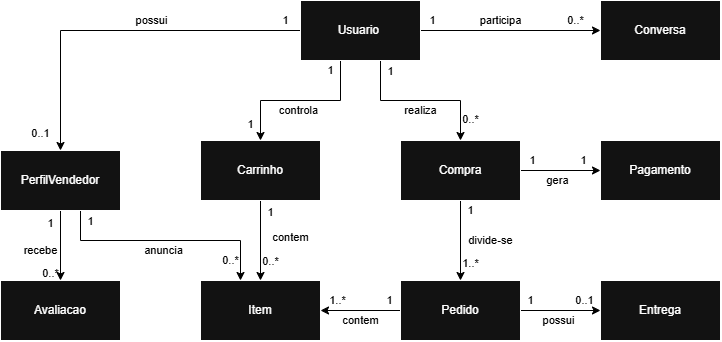
\includegraphics[width=1.1\textwidth, keepaspectratio]{modelo_conceitual_dominio_vp1.drawio.png}
\end{adjustbox}
\caption{Modelo Conceitual de Domínio do Sistema de Brechós (MK1 --- VP1)}
\label{fig:dominio}
\end{figure}

\newpage

\subsection{View de Desenvolvimento (VP2)}

A View de Desenvolvimento detalha a organização lógica do código-fonte estruturada em camadas horizontais bem definidas, conforme as restrições de arquitetura e isolamento de dependências. O Diagrama de Camadas (MK2) explicita os limites de visibilidade direcionais, garantindo o completo isolamento das regras de negócio contidas no núcleo do Domínio em relação às tecnologias de Infraestrutura e Apresentação.

Na materialização física destas camadas, a camada de Apresentação é implementada por templates HTML renderizados no servidor, estilos e assets estáticos em \texttt{apps/front}, HTMX versionado localmente e JavaScript pontual para galeria, uploads e interações específicas. As camadas subjacentes (Aplicação, Domínio e Infraestrutura) são implementadas em Go, garantindo forte tipagem, baixo acoplamento e testes unitários/integrados sobre as regras C2C.

\begin{figure}[H]
\centering
% O adjustbox estica horizontalmente além das margens de texto e re-centraliza simetricamente na folha
\begin{adjustbox}{center}
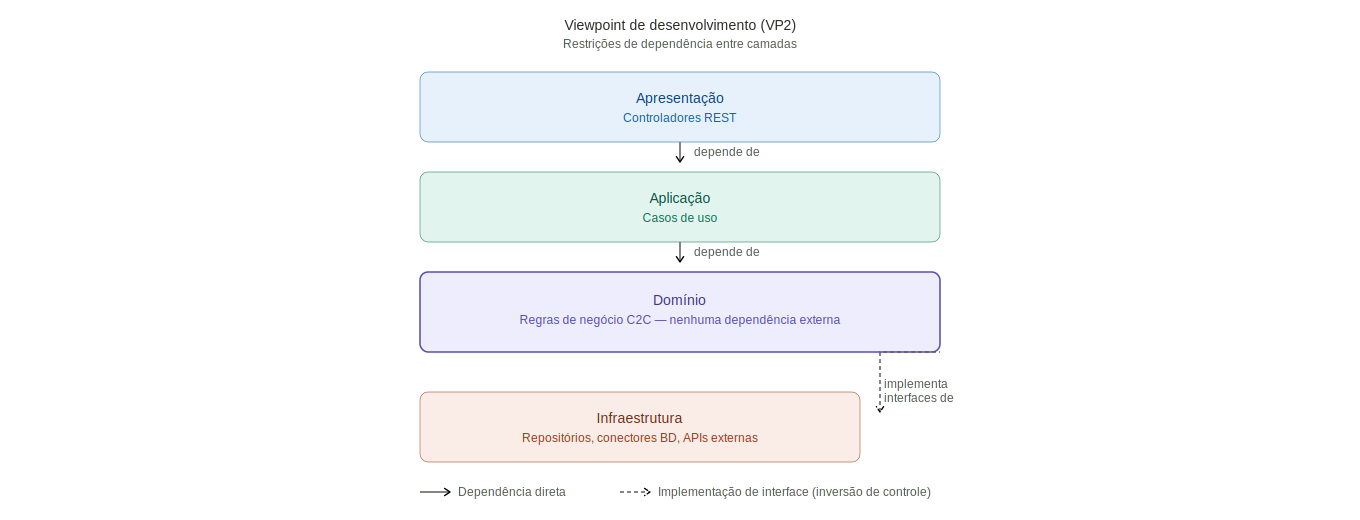
\includegraphics[width=1.25\textwidth, keepaspectratio]{diagrama_camadas.png}
\end{adjustbox}
\caption{Diagrama de Camadas do Sistema de Brechós (MK2 --- VP2)}
\label{fig:camadas}
\end{figure}

\newpage % Isola o próximo diagrama para garantir espaço vertical máximo

% ----------------------------------------
\subsection{View de Implantação (VP4)}

A View de Implantação expõe o mapeamento físico e lógico dos artefatos estruturais do software nos respectivos nós computacionais de execução. Diferente de uma arquitetura \textit{three-tier} tradicional, a infraestrutura adota uma \textbf{Topologia Distribuída em Nuvem (Cloud-Native)}, aproveitando serviços gerenciados (PaaS, DBaaS e \textit{Serverless}) para maximizar a escalabilidade e o isolamento de falhas.

O Diagrama de Implantação (MK3) deve ser interpretado à luz da implementação atual: a apresentação, a API JSON e as páginas SSR são servidas por um único processo Go; o PostgreSQL armazena o estado transacional; o Vercel Blob armazena as imagens públicas dos anúncios; o Mercado Pago processa cobranças quando configurado; o Melhor Envio cota frete quando há credenciais; e o ViaCEP consulta endereços por CEP. Não há contêiner dedicado para WebSocket nem integração com Stripe ou Amazon S3 nesta versão.

\begin{figure}[H]
\centering
\begin{adjustbox}{center}
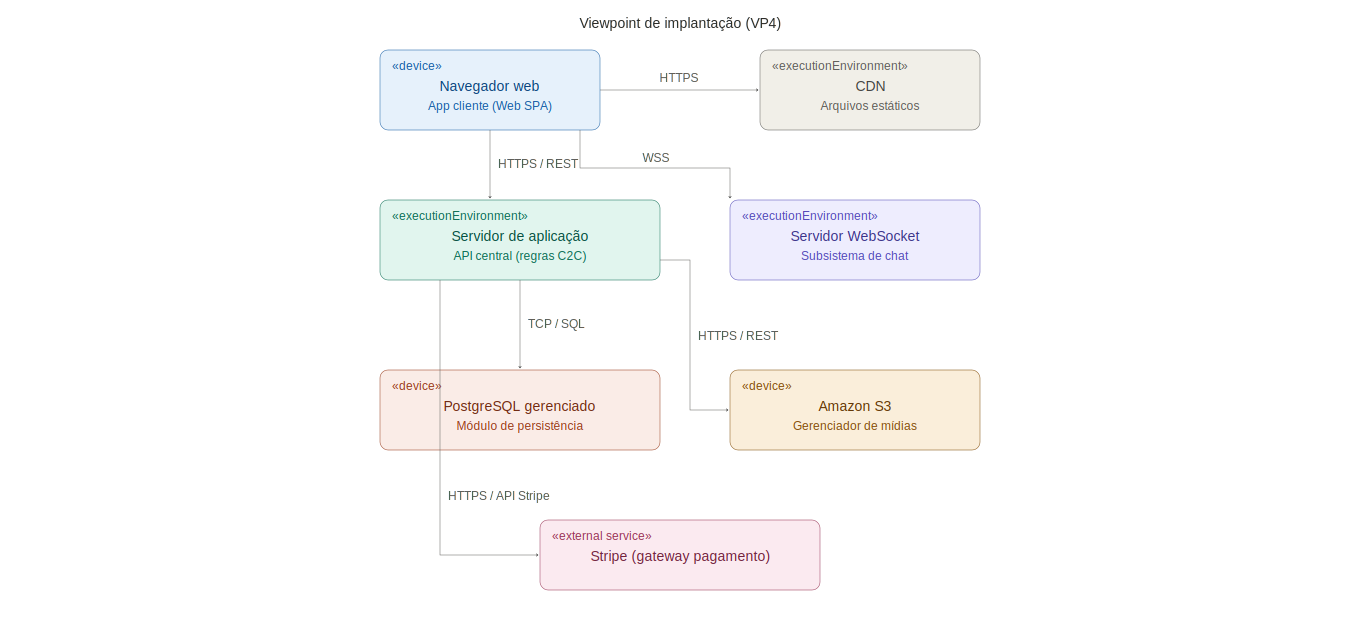
\includegraphics[width=1.25\textwidth, keepaspectratio]{diagrama_implantacao.png}
\end{adjustbox}
\caption{Diagrama de Implantação de Infraestrutura Serverless (MK3 --- VP4)}
\label{fig:implantacao}
\end{figure}

\newpage

% ----------------------------------------
\subsection{View de Cenários (+1)}

A View de Cenários (+1) consolida e valida a arquitetura, demonstrando como os elementos lógicos, de processo e físicos colaboram para entregar as funcionalidades centrais do sistema. A ilustração e validação dos cenários críticos do negócio C2C (como a publicação de um anúncio pelo vendedor e o fluxo transversal de compra) são realizadas por meio de Diagramas de Atividades e de Sequência.

Devido ao seu alto nível de detalhamento de interações, assinaturas de métodos e fluxo de controle estrito, \textbf{estes diagramas compõem formalmente o Documento de Design UML (anexo externo à AD)}, atuando como o elo prático entre esta abstração arquitetural e a implementação técnica das funcionalidades.

\newpage

% ================================================================
% SEÇÃO 5 — ARCHITECTURE DECISIONS E RATIONALE
% ================================================================
\section{Architecture Decisions e Rationale}

Esta seção apresenta as decisões arquiteturais significativas tomadas para o Sistema de Intermediação de Brechós, justificando-as com base nos conceitos de táticas arquiteturais e nos cenários de atributos de qualidade formulados na Seção 2.

\subsection{Decisão 01: Estilo Arquitetural em Camadas (Arquitetura Limpa) e Servidor Stateless}

\noindent\textbf{Decisão:} O sistema adota uma organização lógica estruturada em quatro camadas horizontais rígidas (Apresentação, Aplicação, Domínio e Infraestrutura) sob a ótica da \textbf{Arquitetura Limpa (Clean Architecture)}, empregando o Princípio da Inversão de Dependência, combinada com um modelo de comunicação \textit{stateless} (sem estado) no servidor de aplicação.

\vspace{0.3cm}
\noindent\textbf{Concerns Enquadrados:} CC03 (Manutenibilidade), CQ02 (Escalabilidade) e CQ04 (Disponibilidade).

\vspace{0.3cm}
\noindent\textbf{Rationale (Justificativa):} 
\begin{itemize}
    \item \textbf{Uso de Camadas e Arquitetura Limpa (CC03):} A imposição de restrições de visibilidade estritas entre as camadas isola as regras de negócio das tecnologias de infraestrutura. A adoção da Inversão de Controle força a Infraestrutura a depender do Domínio, protegendo o núcleo do negócio de mudanças em APIs externas e bancos de dados, alinhando-se aos princípios mais modernos de isolamento. Isso reduz o acoplamento global, permitindo modificações isoladas em componentes específicos (como a troca de bibliotecas na camada de Apresentação) sem causar efeitos colaterais na lógica de domínio, o que atende diretamente ao interesse de manutenibilidade da equipe de desenvolvimento.
    \item \textbf{Estruturação Stateless (CQ02 e CQ04):} O backend Go não mantém estado de sessão em memória. A sessão web é transportada por cookie seguro e os dados permanentes ficam no PostgreSQL. Essa separação permite reiniciar ou replicar o processo de aplicação sem perder sessões persistidas ou dados transacionais, desde que as instâncias compartilhem o mesmo banco e as mesmas chaves de configuração.
\end{itemize}

\noindent\textbf{Trade-offs e Riscos:} A introdução de camadas intermediárias adiciona uma pequena latência no tempo de resposta (\textit{overhead} de chamadas de métodos e mapeamentos entre objetos de diferentes camadas). A opção por um processo Go único simplifica a operação acadêmica, mas exige cuidado futuro para escalar horizontalmente, configurar proxy reverso confiável, compartilhar segredos de sessão e monitorar o PostgreSQL.

% ----------------------------------------
\subsection{Decisão 02: Padrão de Persistência com Data Mapper}

\noindent\textbf{Decisão:} Isolamento da persistência de dados através do padrão \textit{Data Mapper}, separando completamente as entidades puras do domínio das tabelas e esquemas relacionais do banco de dados PostgreSQL.

\vspace{0.3cm}
\noindent\textbf{Concerns Enquadrados:} CC03 (Manutenibilidade e Evolvabilidade) e CC02 (Viabilidade de Construção).

\vspace{0.3cm}
\noindent\textbf{Rationale (Justificativa):} 
Diferente do padrão \textit{Active Record} (onde a lógica de banco de dados fica misturada com a lógica de negócio), o \textit{Data Mapper} permite que as regras complexas do ciclo de vida de pedidos e anúncios do brechó permaneçam agnósticas em relação ao banco de dados. Isso viabiliza a criação de testes unitários robustos e independentes da infraestrutura física, acelerando o ciclo de desenvolvimento em ambiente acadêmico (CC02). Além disso, mudanças na modelagem física do PostgreSQL impactam apenas o arquivo de mapeamento da infraestrutura, protegendo a integridade do núcleo do sistema.

\vspace{0.3cm}
\noindent\textbf{Trade-offs:} O isolamento provido pelo \textit{Data Mapper} exige um rigoroso \textit{trade-off} com o Desempenho (CQ01). A separação estrita entre o Domínio e a Infraestrutura adiciona um \textit{overhead} de processamento para realizar o mapeamento e a tradução constante entre os objetos da aplicação e as tabelas relacionais, além de exigir que a equipe escreva um volume maior de código inicial (\textit{boilerplate}).

% ----------------------------------------
\subsection{Decisão 03: SSR com HTMX e Comunicação por HTTP}

\noindent\textbf{Decisão:} Adoção de renderização no servidor (SSR) com templates Go e melhoria progressiva via HTMX, mantendo a navegação, formulários, conversas e notificações sobre requisições HTTP convencionais. O frontend não possui etapa de build, não usa runtime SPA e mantém JavaScript próprio apenas para interações locais específicas.

\vspace{0.3cm}
\noindent\textbf{Concerns Enquadrados:} CQ01 (Desempenho), CQ03 (Segurança), CQ04 (Disponibilidade) e CC02 (Viabilidade).

\vspace{0.3cm}
\noindent\textbf{Rationale (Justificativa):} 
O uso de SSR/HTMX reduziu a complexidade de build e implantação, facilitou a validação acadêmica e manteve as URLs navegáveis com HTML convencional. Como a sessão fica em cookie \textit{HttpOnly}, o token não é exposto ao JavaScript nem persistido em Web Storage. A mesma aplicação Go atende as páginas HTML e a API JSON, reaproveitando os mesmos controladores de casos de uso e reduzindo duplicidade entre camadas.

\vspace{0.3cm}
\noindent\textbf{Trade-offs e Sensibilidade:} A ausência de WebSocket reduz a infraestrutura e o consumo de conexões persistentes, mas torna a comunicação menos imediata que uma solução \textit{full-duplex}. Para o escopo implementado, a conversa por pedido e as notificações por HTTP/HTMX atendem ao fluxo acadêmico sem servidor adicional.

% ----------------------------------------
\subsection{Decisão 04: Stack Tecnológica de Implementação (Go, SSR/HTMX e PostgreSQL)}

\noindent\textbf{Decisão:} Adoção da linguagem Go para backend, casos de uso, domínio, adaptadores HTTP/SSR e migrações; HTMX e templates Go para a camada de apresentação; PostgreSQL como banco relacional; Vercel Blob para arquivos; Mercado Pago, Melhor Envio e ViaCEP como integrações externas.

\vspace{0.3cm}
\noindent\textbf{Concerns Enquadrados:} CQ01 (Desempenho), CQ02 (Escalabilidade) e CC02 (Viabilidade de Construção).

\vspace{0.3cm}
\noindent\textbf{Rationale (Justificativa):} 
A linguagem Go foi selecionada por sua simplicidade operacional, forte tipagem, bom desempenho e biblioteca padrão robusta para HTTP. A combinação SSR/HTMX evita a complexidade de um frontend SPA, reduz dependências e permite que os mesmos controladores atendam HTML e JSON. O PostgreSQL foi mantido como fonte transacional de verdade, enquanto Vercel Blob evita armazenar binários no banco. Mercado Pago, Melhor Envio e ViaCEP refletem provedores adequados ao contexto brasileiro do sistema.

\vspace{0.3cm}
\noindent\textbf{Trade-offs:} SSR/HTMX reduz a autonomia de uma SPA rica e exige cuidado com templates e fragmentos HTML. As integrações reais ainda possuem limitações: pagamentos e reembolsos têm fallback simulado, o split/repasse ao vendedor não está completo e a limpeza de imagens órfãs permanece como melhoria futura.

% ================================================================
% SEÇÃO 6 — CORRESPONDENCES E CORRESPONDENCE RULES
% ================================================================
\section{Correspondences e Correspondence Rules}

Conforme estabelecido pela ISO/IEC/IEEE 42010:2022, as \textit{Correspondences} (Correspondências) expressam as relações entre os elementos arquiteturais presentes em diferentes \textit{Architecture Views}, enquanto as \textit{Correspondence Rules} (Regras de Correspondência) definem as restrições e invariantes que governam essas relações. 

O objetivo desta seção é garantir a consistência global e auditar a \textit{Architecture Description}, assegurando rastreabilidade de ponta a ponta: desde as exigências de negócio e restrições de qualidade (Seção 2), passando pelas decisões técnicas tomadas (Seção 5), até a materialização nos artefatos de código e topologia física (Seção 4). Isso previne a erosão arquitetural durante o ciclo de desenvolvimento.

\subsection{Regras de Correspondência (Correspondence Rules)}

As seguintes regras normativas foram estipuladas para governar a arquitetura do Sistema de Intermediação de Brechós.

\begin{itemize}[noitemsep]
    \item \textbf{CR-01 (Completude e Alocação de Implantação):} Todo componente de software lógico mapeado e estruturado nos viewpoints deve possuir rastreabilidade exata para pelo menos um nó de execução no Diagrama de Implantação (VP4). Nenhum artefato de software pode existir flutuando sem um contêiner ou ambiente de hospedagem físico associado. 
    
    \item \textbf{CR-02 (Cobertura de Atributos de Qualidade):} Todo concern de qualidade priorizado (CQ01 a CQ04) deve estar fundamentado e mitigado por, no mínimo, uma Decisão Arquitetural documentada (Seção 5). 
    \textit{Validação: Matriz de Rastreabilidade Qualidade-Decisão (Seção 6.2.1).}
    
    \item \textbf{CR-03 (Isolamento de Domínio e Inversão de Controle):} No Viewpoint de Desenvolvimento (VP2), os artefatos contidos na camada de \textbf{Domínio} (regras de intermediação C2C, ciclo de vida de pedidos) estão expressamente proibidos de acoplar dependências externas (APIs HTTP, conectores PostgreSQL). A injeção de dependência deve ser utilizada para inverter o controle, forçando a camada de Infraestrutura a implementar as interfaces definidas pelo Domínio.
    \textit{Validação: Revisão de código (\textit{Pull Requests}) garantindo a ausência de \textit{imports} de infraestrutura nas classes de entidade.}
    
    \item \textbf{CR-04 (Delegação Financeira Restrita):} Nenhum componente interno do sistema está autorizado a persistir ou trafegar dados completos de cartões de crédito (PAN, CVV) no banco de dados da aplicação. O fluxo deve empregar \textit{tokens} opacos gerados no \textit{frontend} e enviados diretamente ao \textit{Gateway} de Pagamento.
    \textit{Validação: Auditoria no mapeamento físico do banco de dados (esquema SQL).}
\end{itemize}

\subsection{Correspondências Identificadas (Correspondences)}

As matrizes a seguir formalizam a aplicação prática das regras definidas, evidenciando a consistência e a integridade desta \textit{Architecture Description}.

\subsubsection{Mapeamento de Concerns para Decisões Arquiteturais (Aplica CR-02)}

Esta matriz comprova que as restrições não funcionais do sistema foram ativamente resolvidas através de táticas arquiteturais concretas.

\begin{longtable}{|p{2cm}|p{3.5cm}|p{8.5cm}|}
\hline
\textbf{ID / Concern} & \textbf{Atributo Alvo} & \textbf{Decisão Arquitetural e Tática de Mitigação} \\
\hline
\endfirsthead
\hline
\textbf{ID / Concern} & \textbf{Atributo Alvo} & \textbf{Decisão Arquitetural e Tática de Mitigação} \\
\hline
\endhead
\textbf{CQ01} & Desempenho & \textbf{Decisão 01, 03 e 04:} Uso de Go, SSR/HTMX, paginação do catálogo e processamento transacional do checkout para reduzir complexidade e manter respostas previsíveis. \\
\hline
\textbf{CQ02} & Escalabilidade & \textbf{Decisão 01 e 04:} Aplicação sem sessão em memória local, persistência centralizada no PostgreSQL, imagens fora do banco no Vercel Blob e listagens paginadas. \\
\hline
\textbf{CQ03} & Segurança & \textbf{Decisão 01, 03 e CR-04:} Sessão por cookie \textit{HttpOnly}, verificação de origem contra CSRF, não armazenamento de PAN/CVV e tokenização de cartão via Mercado Pago quando o pagamento real está habilitado. \\
\hline
\textbf{CQ04} & Disponibilidade & \textbf{Decisão 03 e 04:} Uso de endpoints de saúde, fallback de frete fixo, provedor de pagamento simulado sem credenciais e jobs periódicos para expirar reservas e prazos de envio. \\
\hline
\textbf{CC03} & Manutenibilidade & \textbf{Decisão 02 e CR-03:} Uso rigoroso do padrão \textit{Data Mapper}. Permite que a lógica central do brechó seja testada de forma unitária, acelerando a identificação de falhas e refatorações. \\
\hline
\end{longtable}

\subsubsection{Rastreabilidade Lógica vs. Física de Implantação (Aplica CR-01)}

A matriz a seguir demonstra a alocação dos elementos lógicos nos respectivos nós de infraestrutura necessários para a operação do sistema web.

\begin{longtable}{|p{4cm}|p{5cm}|p{5cm}|}
\hline
\textbf{Elemento Lógico} & \textbf{Nó de Execução (VP4)} & \textbf{Relação Semântica} \\
\hline
\endfirsthead
\hline
\textbf{Elemento Lógico} & \textbf{Nó de Execução (VP4)} & \textbf{Relação Semântica} \\
\hline
\endhead
Páginas SSR/HTMX & Processo Go da aplicação e navegador Web & \textit{Is rendered by} (HTML gerado no servidor e melhorado progressivamente no cliente) \\
\hline
Serviço de Arquivos Estáticos & Processo Go da aplicação & \textit{Is hosted on} (Responsável por entregar CSS, JavaScript local, logos e assets) \\
\hline
API Central (Regras C2C) & Processo Go da aplicação & \textit{Is deployed on} (Processa cadastro, anúncios, carrinho, checkout, pedidos, vendas, notificações e conversas) \\
\hline
Subsistema de Conversas e Notificações & Processo Go e PostgreSQL & \textit{Reads/Writes to} (Persiste mensagens/notificações e renderiza atualizações por HTTP/HTMX) \\
\hline
Módulo de Persistência & PostgreSQL & \textit{Reads/Writes to} (Garante o armazenamento permanente e ACID das entidades) \\
\hline
Gerenciador de Mídias & Vercel Blob & \textit{Communicates with} (Armazena e distribui as fotos públicas dos anúncios) \\
\hline
Integrações de Negócio & Mercado Pago, Melhor Envio e ViaCEP & \textit{Communicates with} (Processa cobranças, cota frete e consulta CEP) \\
\hline
\end{longtable}

\subsubsection{Matriz de Restrição de Dependência de Camadas (Aplica CR-03)}

Para garantir que a manutenibilidade não seja corrompida por acoplamento indevido, a arquitetura estabelece um vetor direcional estrito de dependências. A tabela abaixo mapeia as relações permitidas entre as camadas do \textit{backend}.

\begin{longtable}{|p{3.5cm}|p{10.5cm}|}
\hline
\textbf{Camada Origem} & \textbf{Pode depender e importar recursos da(s) Camada(s) Destino} \\
\hline
\endfirsthead
\hline
\textbf{Camada Origem} & \textbf{Pode depender e importar recursos da(s) Camada(s) Destino} \\
\hline
\endhead
\textbf{Apresentação} (Controladores Rest) & Camada de Aplicação (Casos de Uso) \\
\hline
\textbf{Aplicação} (Casos de Uso) & Camada de Domínio (Entidades e Interfaces) \\
\hline
\textbf{Infraestrutura} (Repositórios) & Camada de Domínio (Implementa as Interfaces do Domínio) \\
\hline
\textbf{Domínio} (Regras de Negócio C2C) & \textbf{NENHUMA.} (O Domínio é puro e isolado de todas as outras camadas). \\
\hline
\end{longtable}

\end{document}
